\graphicspath{{images/}}

\section{Методы приближения функций}

\subsection{Полиномиальная интерполяция}

\subsubsection{Постановка задачи}
Используя таблицу значений $Y_i$ функции $y = f(x)$, вычисленных в точках $X_i$, $i = 0, \dots ,3$  построить интерполяционные многочлены Лагранжа и Ньютона, проходящие через точки $\{X_i, Y_i\}$. Вычислить значение погрешности интерполяции в точке $X^*$.

\subsubsection{Консоль}
\begin{alltt}
4
-0.4 -0.1 0.2 0.5
0.1
Интерполяционный многочлен Лагранжа: 7.55373e-05 + 1.99923 * x + 0.00197657 * x^2 + 0.188516 * x^3
Погрешность в точке Х*: 0.000111543
Интерполяционный многочлен Ньютона: 7.55373e-05 + 1.99923 * x + 0.00197657 * x^2 + 0.188516 * x^3
Погрешность в точке Х*: 0.000111543
\end{alltt}

\subsubsection{Исходный код}
\lstinputlisting{../../NM3_1/interpolation.h}
\pagebreak

\subsection{Сплай-интерполяция}

\subsubsection{Постановка задачи}
Построить кубический сплайн для функции, заданной в узлах интерполяции,
предполагая, что сплайн имеет нулевую кривизну при $x = x_0$ и $x = x_4$. Вычислить значение функции в точке $x = X^*$.

\subsubsection{Консоль}
\begin{alltt}
5
-0.4 -0.1 0.2 0.5 0.8
-0.81152 -0.20017 0.40136 1.0236 1.7273
0.1
Сплайн: i = 1, a = -0.81152, b = 2.04668, c = 0.00000,d = -0.09833
i = 2, a = -0.20017, b = 2.02013, c = -0.08850,d = 0.12796
i = 3, a = 0.40136, b = 2.00158, c = 0.02667,d = 0.71722
i = 4, a = 1.02360, b = 2.21123, c = 0.67217,d = -0.74685

Значение в точке X*: 0.20134
\end{alltt}
\pagebreak

\subsubsection{Результат}
\begin{center}
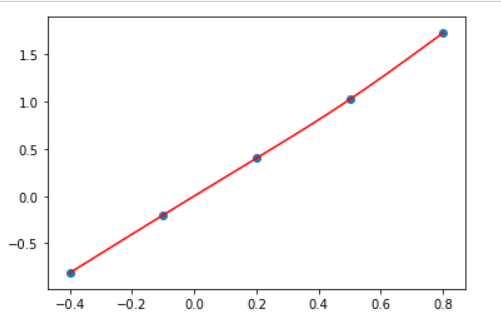
\includegraphics[scale=0.75]{3-2spline}
\end{center}
\pagebreak

\subsubsection{Исходный код}
\lstinputlisting{../../NM3_2/spline.h}
\pagebreak

\subsection{Метод наименьших квадратов}

\subsubsection{Постановка задачи}
Для таблично заданной функции путем решения нормальной системы МНК найти приближающие многочлены a) 1-ой и б) 2-ой степени. Для каждого из приближающих многочленов вычислить сумму квадратов ошибок. Построить графики приближаемой функции и приближающих многочленов.

\subsubsection{Консоль}
\begin{alltt}
6
-0.7 -0.4 -0.1 0.2 0.5 0.8
-1.4754 -0.81152 -0.20017 0.40136 1.0236 1.7273
Приближающий многочлен первой степени: 0.00553 2.10670
Сумма квадратов ошибок: 0.00394
Приближающий многочлен второй степени: 0.00553 2.10670 0.00000
Сумма квадратов ошибок: 0.00394
\end{alltt}
\pagebreak

\subsubsection{Результат}
\begin{center}
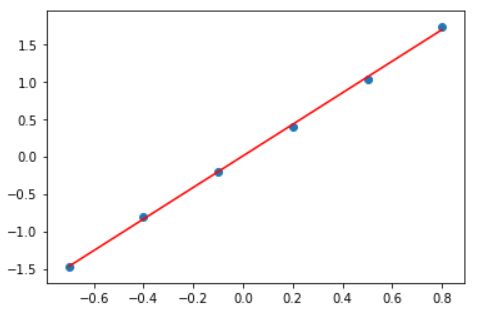
\includegraphics[scale=0.75]{3-3ms}
\end{center}
\pagebreak

\subsubsection{Исходный код}
\lstinputlisting{../../NM3_3/MNK.h}
\pagebreak

\subsection{Численное дифференцирование}

\subsubsection{Постановка задачи}
Вычислить первую и вторую производную от таблично заданной функции $y_i = f(x_i)$, $i = 0, 1, 2, 3, 4$ в точке $x = X^*$.

\subsubsection{Консоль}
\begin{alltt}
5
-1.0 0.0 1.0 2.0 3.0
-1.7854 0.0 1.7854 3.1071 4.249
1
Первая производная функции в точке x0 = 1.0000, f'(x0) = 1.7854
Вторая производная функции в точке x0 = 1.0000, f''(x0) = 0.0000
\end{alltt}
\pagebreak

\subsubsection{Исходный код}
\lstinputlisting{../../NM3_4/table_function.h}
\pagebreak

\subsection{Численное интегрирование}

\subsubsection{Постановка задачи}
Вычислить определенный интеграл $F = \int_{X_0}^{X_1}{y dx}$, методами прямоугольников, трапеций, Симпсона с шагами $h_1$, $h_2$. Оценить погрешность вычислений, используя Метод Рунге-Ромберга:

\subsubsection{Консоль}
\begin{alltt}
0 4 1.0 0.5
Метод прямоугольников с шагом 1: 0.040489
Метод трапеций с шагом 1: 0.046395
Метод Симпсона с шагом 1: 0.0141526

Метод прямоугольников с шагом 0.5: 0.0418683
Метод трапеций с шагом 0.5: 0.043442
Метод Симпсона с шагом 0.5: 0.014131

Погрешность вычислений методом прямоугольников: 0.00183909
Погрешность вычислений методом трапеций: 0.00393738
Погрешность вычислений методом Симпсона: 2.304e-05
\end{alltt}
\pagebreak

\subsubsection{Исходный код}
\lstinputlisting{../../NM3_5/integrate.h}
\pagebreak
